% Options for packages loaded elsewhere
\PassOptionsToPackage{unicode}{hyperref}
\PassOptionsToPackage{hyphens}{url}
%
\documentclass[
  man,floatsintext]{apa6}
\usepackage{amsmath,amssymb}
\usepackage{iftex}
\ifPDFTeX
  \usepackage[T1]{fontenc}
  \usepackage[utf8]{inputenc}
  \usepackage{textcomp} % provide euro and other symbols
\else % if luatex or xetex
  \usepackage{unicode-math} % this also loads fontspec
  \defaultfontfeatures{Scale=MatchLowercase}
  \defaultfontfeatures[\rmfamily]{Ligatures=TeX,Scale=1}
\fi
\usepackage{lmodern}
\ifPDFTeX\else
  % xetex/luatex font selection
\fi
% Use upquote if available, for straight quotes in verbatim environments
\IfFileExists{upquote.sty}{\usepackage{upquote}}{}
\IfFileExists{microtype.sty}{% use microtype if available
  \usepackage[]{microtype}
  \UseMicrotypeSet[protrusion]{basicmath} % disable protrusion for tt fonts
}{}
\makeatletter
\@ifundefined{KOMAClassName}{% if non-KOMA class
  \IfFileExists{parskip.sty}{%
    \usepackage{parskip}
  }{% else
    \setlength{\parindent}{0pt}
    \setlength{\parskip}{6pt plus 2pt minus 1pt}}
}{% if KOMA class
  \KOMAoptions{parskip=half}}
\makeatother
\usepackage{xcolor}
\usepackage{graphicx}
\makeatletter
\def\maxwidth{\ifdim\Gin@nat@width>\linewidth\linewidth\else\Gin@nat@width\fi}
\def\maxheight{\ifdim\Gin@nat@height>\textheight\textheight\else\Gin@nat@height\fi}
\makeatother
% Scale images if necessary, so that they will not overflow the page
% margins by default, and it is still possible to overwrite the defaults
% using explicit options in \includegraphics[width, height, ...]{}
\setkeys{Gin}{width=\maxwidth,height=\maxheight,keepaspectratio}
% Set default figure placement to htbp
\makeatletter
\def\fps@figure{htbp}
\makeatother
\setlength{\emergencystretch}{3em} % prevent overfull lines
\providecommand{\tightlist}{%
  \setlength{\itemsep}{0pt}\setlength{\parskip}{0pt}}
\setcounter{secnumdepth}{-\maxdimen} % remove section numbering
% Make \paragraph and \subparagraph free-standing
\ifx\paragraph\undefined\else
  \let\oldparagraph\paragraph
  \renewcommand{\paragraph}[1]{\oldparagraph{#1}\mbox{}}
\fi
\ifx\subparagraph\undefined\else
  \let\oldsubparagraph\subparagraph
  \renewcommand{\subparagraph}[1]{\oldsubparagraph{#1}\mbox{}}
\fi
\newlength{\cslhangindent}
\setlength{\cslhangindent}{1.5em}
\newlength{\csllabelwidth}
\setlength{\csllabelwidth}{3em}
\newlength{\cslentryspacingunit} % times entry-spacing
\setlength{\cslentryspacingunit}{\parskip}
\newenvironment{CSLReferences}[2] % #1 hanging-ident, #2 entry spacing
 {% don't indent paragraphs
  \setlength{\parindent}{0pt}
  % turn on hanging indent if param 1 is 1
  \ifodd #1
  \let\oldpar\par
  \def\par{\hangindent=\cslhangindent\oldpar}
  \fi
  % set entry spacing
  \setlength{\parskip}{#2\cslentryspacingunit}
 }%
 {}
\usepackage{calc}
\newcommand{\CSLBlock}[1]{#1\hfill\break}
\newcommand{\CSLLeftMargin}[1]{\parbox[t]{\csllabelwidth}{#1}}
\newcommand{\CSLRightInline}[1]{\parbox[t]{\linewidth - \csllabelwidth}{#1}\break}
\newcommand{\CSLIndent}[1]{\hspace{\cslhangindent}#1}
\ifLuaTeX
\usepackage[bidi=basic]{babel}
\else
\usepackage[bidi=default]{babel}
\fi
\babelprovide[main,import]{english}
% get rid of language-specific shorthands (see #6817):
\let\LanguageShortHands\languageshorthands
\def\languageshorthands#1{}
% Manuscript styling
\usepackage{upgreek}
\captionsetup{font=singlespacing,justification=justified}

% Table formatting
\usepackage{longtable}
\usepackage{lscape}
% \usepackage[counterclockwise]{rotating}   % Landscape page setup for large tables
\usepackage{multirow}		% Table styling
\usepackage{tabularx}		% Control Column width
\usepackage[flushleft]{threeparttable}	% Allows for three part tables with a specified notes section
\usepackage{threeparttablex}            % Lets threeparttable work with longtable

% Create new environments so endfloat can handle them
% \newenvironment{ltable}
%   {\begin{landscape}\centering\begin{threeparttable}}
%   {\end{threeparttable}\end{landscape}}
\newenvironment{lltable}{\begin{landscape}\centering\begin{ThreePartTable}}{\end{ThreePartTable}\end{landscape}}

% Enables adjusting longtable caption width to table width
% Solution found at http://golatex.de/longtable-mit-caption-so-breit-wie-die-tabelle-t15767.html
\makeatletter
\newcommand\LastLTentrywidth{1em}
\newlength\longtablewidth
\setlength{\longtablewidth}{1in}
\newcommand{\getlongtablewidth}{\begingroup \ifcsname LT@\roman{LT@tables}\endcsname \global\longtablewidth=0pt \renewcommand{\LT@entry}[2]{\global\advance\longtablewidth by ##2\relax\gdef\LastLTentrywidth{##2}}\@nameuse{LT@\roman{LT@tables}} \fi \endgroup}

% \setlength{\parindent}{0.5in}
% \setlength{\parskip}{0pt plus 0pt minus 0pt}

% Overwrite redefinition of paragraph and subparagraph by the default LaTeX template
% See https://github.com/crsh/papaja/issues/292
\makeatletter
\renewcommand{\paragraph}{\@startsection{paragraph}{4}{\parindent}%
  {0\baselineskip \@plus 0.2ex \@minus 0.2ex}%
  {-1em}%
  {\normalfont\normalsize\bfseries\itshape\typesectitle}}

\renewcommand{\subparagraph}[1]{\@startsection{subparagraph}{5}{1em}%
  {0\baselineskip \@plus 0.2ex \@minus 0.2ex}%
  {-\z@\relax}%
  {\normalfont\normalsize\itshape\hspace{\parindent}{#1}\textit{\addperi}}{\relax}}
\makeatother

\makeatletter
\usepackage{etoolbox}
\patchcmd{\maketitle}
  {\section{\normalfont\normalsize\abstractname}}
  {\section*{\normalfont\normalsize\abstractname}}
  {}{\typeout{Failed to patch abstract.}}
\patchcmd{\maketitle}
  {\section{\protect\normalfont{\@title}}}
  {\section*{\protect\normalfont{\@title}}}
  {}{\typeout{Failed to patch title.}}
\makeatother

\usepackage{xpatch}
\makeatletter
\xapptocmd\appendix
  {\xapptocmd\section
    {\addcontentsline{toc}{section}{\appendixname\ifoneappendix\else~\theappendix\fi\\: #1}}
    {}{\InnerPatchFailed}%
  }
{}{\PatchFailed}
\keywords{Depression; Mental Health\newline\indent Word count: 2571}
\usepackage{csquotes}
\ifLuaTeX
  \usepackage{selnolig}  % disable illegal ligatures
\fi
\IfFileExists{bookmark.sty}{\usepackage{bookmark}}{\usepackage{hyperref}}
\IfFileExists{xurl.sty}{\usepackage{xurl}}{} % add URL line breaks if available
\urlstyle{same}
\hypersetup{
  pdftitle={Exploring the Gender Difference in Depression Severity and Depressive Symptoms in Chinese Adolescents},
  pdfauthor={Annika Liu1 \& Xiwang Fan2},
  pdflang={en-EN},
  pdfkeywords={Depression; Mental Health},
  hidelinks,
  pdfcreator={LaTeX via pandoc}}

\title{Exploring the Gender Difference in Depression Severity and Depressive Symptoms in Chinese Adolescents}
\author{Annika Liu\textsuperscript{1} \& Xiwang Fan\textsuperscript{2}}
\date{}


\shorttitle{Clinical depression in Chinese adolescents}

\authornote{

Add complete departmental affiliations for each author here. Each new line herein must be indented, like this line.

Enter author note here.

The authors made the following contributions. Annika Liu: Conceptualization, Writing - Original Draft Preparation, Writing - Review \& Editing; Xiwang Fan: Supervision.

Correspondence concerning this article should be addressed to Annika Liu, Postal address. E-mail: \href{mailto:my@email.com}{\nolinkurl{my@email.com}}

}

\affiliation{\phantom{0}}

\abstract{%
This report is part of a comprehensive study on depression among Chinese adolescents, encompassing an analysis of 577 eligible participants aged 10 to 19 years, all with HAMD total scores of 8 or higher. Focused on a specific aspect of a larger, long-term project, this report examines gender differences in depression severity and in three key symptom factors: somatization/anxiety, cognitive impairment, and hopelessness. Chinese version of HAMD-24 was used in this study. A linear regression analysis was performed to show the general picture and explore gender differences on overall depression scores. Furthermore, four t-tests were employed to identify gender differences in the total depression score once again, as well as examining the gender role in each of the three symptom factors. The results of our study indicate that among Chinese adolescents, females exhibit greater depression severity and more intense symptoms of cognitive impairment and hopelessness than their male counterparts. The objective of this report is to make a substantial contribution to our broader ongoing research on adolescent depression in China, thereby deepening insights into the gender-based variations in these conditions and informing clinical approaches.
}



\begin{document}
\maketitle

\hypertarget{introducation}{%
\section{Introducation}\label{introducation}}

Depression is the one of the principal causes of illness and disability in the world(NIMH, 2023). The World Health Organization (WHO) has been issuing warnings about this pathology for years, given that it affects over 300 million people all over the world(WHO, 2017). Meanwhile, depression is highly prevalent in adolescence (NIMH, 2023).According to WHO, adolescence ranges from 10 to 19 years old is an important developmental period marked by formative biological and social transition (Blakemore \& Mills, 2014). Experiencing depression or any kind of mental health struggle during this period can disrupt these essential processes, which ultimately can affect an individual's long-term socioeconomic standing and peer, familial, and romantic relationships, causing but not limited to failure to complete secondary school, unemployment, and pregnancy/parenthood (Clayborne, Varin, \& Colman, 2019). Researchers indicated that considering the high rates of depressed mood, depressive syndromes, and depressive disorders that occur during adolescence, treatment and research efforts will never be sufficient to meet the full needs of the population (Nolen-Hoeksema \& Hilt, 2013).

Chinese adolescents' mental health has received attention from scholars in recent years. Studies have shown that adolescents in China experience emotional disturbances, including depression, at levels equal to or greater than their American peers (Hesketh \& Ding, 2005). Quach, Epstein, Riley, Falconier, and Fang (2015) analyzed in their research that this may be due to society's emphasis on academic achievement and its close association with financial success and social status. The current research provided a detailed analysis of adolescent depression and related symptoms in this culturally specific context. The hope is to raise awareness among more people, including governments, educational institutions, and parents, about these issues within the context of a high-pressure culture, contributing to more targeted solutions for Chinese adolescents.

Notable gender differences in terms of both depression prevalence and clinical symptoms were found, highlighting women were approximately twice as likely as men to suffer from this mental disorder(Jung, Cho, \& Kim, 2019; Nolen-Hoeksema, 1990). Similar findings have been discovered in research focused on adolescents, revealing that adolescent females are also exposed to a greater vulnerability to depression(Lewis et al., 2015). Specifically, Sun and his colleagues in a study targeting Chinese adolescents indicated that female adolescents in China exhibit a higher prevalence and severity of depressive symptoms, such as insomnia (Sun et al., 2023).

\hypertarget{current-study}{%
\subsection{Current Study}\label{current-study}}

Expanding upon prior research into depression among Chinese adolescents (Sun et al., 2023), the present study aims to investigate and analyze gender disparities in the severity of depression and three associated symptoms, including somatization/anxiety, cognitive impairment, and hopelessness. According to the above discussion of gender differences, we predict that Chinese female adolescents with depression would have a more severe degree of depression, represented by a higher depression score.

In the context of somatization/anxiety, Hamilton asserted that some patients may exhibit a paradox of depression, characterized by an absence of depressed mood, underscoring the significance of somatic symptoms, such as perceived body pain and hypochondriasis, in the diagnosis of depression (Lipowski, 1990). The somatization/anxiety dimension utilized in this study is identified as one of the factors in the HAMD-24, details of which will be elaborated in the methods section. A study among high school students revealed a substantial gender difference in the prevalence of anxious somatic depression, with females reporting higher rates (Silverstein, Caceres, Perdue, \& Cimarolli, 1995). Building on this finding, our study anticipates observing a similar gender disparity, that females tend to have a higher somatization/anxiety score, among Chinese adolescents aged 10-19 who have been diagnosed with depression.

Cognitive impairment, also sometimes termed cognitive dysfunction, encompasses difficulties with attention, learning, short-term and working memory, problem-solving capabilities, processing speed, and motor function (Lam, Kennedy, McIntyre, \& Khullar, 2014). Such impairments are often linked to cognitive-affective bias, leading to skewed information processing and atypical reactions to negative feedback and decision-making (Lam et al., 2014). Presently, research focusing on adult populations has not definitively demonstrated a gender disparity in cognitive impairment among patients with depression (Lv et al., 2023). However, considering that women generally report more severe symptoms of depression, and taking into account different sample age ranges from Lv et al. (2023)'s pervious study, we anticipate that cognitive impairment will be more pronounced in female adolescents.

Hopelessness is characterized by pessimistic expectations regarding future situations and events (Alloy \& Ahrens, 1987). Beck, Steer, Beck, and Newman (1993) regarded hopelessness as the third element of his cognitive negative triad of depression, which encompasses the self and the external environment, as well as a significant risk factor for suicide. Furthermore, a study conducted during the COVID-19 pandemic on the mental health of adolescents reported that moderate to severe hopelessness was more prevalent among adolescent females than males(Takács, Katona, \& Ihász, 2023). Following this, our study hypothesizes a similar picture that among Chinese adolescents with depression, females will exhibit higher levels of hopelessness.

This study, as part of a large-scale investigation into adolescent depression in China, aims to explore the manifestation of gender differences in the severity of depression and three specific depressive symptoms. It hopes to contribute to a more comprehensive understanding of this condition within the cultural and regional context of China and to propose more gender-targeted treatment approaches in the field of clinical psychology.

\hypertarget{method}{%
\section{Method}\label{method}}

\hypertarget{participants}{%
\subsection{Participants}\label{participants}}

Participants were recruited between March 2021 and June 2023 from the Mental Health Center of Tongji University Psychological Assessment and Research Center in Shanghai. They underwent structured psychiatric interviews administered by trained psychiatrists at the health center, who utilized the formally translated Chinese version of the 24-item Hamilton depression rating scale (HAMD-24)(Hamilton, 1960). This standardized assessment tool is widely recognized and accepted within the professional field. Eligible participants for this study specifically had to satisfy the following inclusionary criteria: (1) adolescents aged between 10 and 19 years old; (2) HAMD-24 score bigger or equal to 8. A total of 577 adolescent participants were included (Female = 436; Male = 141). There were no exclusion criteria. The terms `Male' and `Female' are employed to denote the binary sexes of participants, referring to the biological attributes assigned at birth based on physical anatomy and physiological characteristics (Heidari, Babor, De Castro, Tort, \& Curno, 2016) The Institutional Review Board (Medical Ethics Committee of Shanghai Pudong New Area Mental Health Center) approved the study (Ethical approval number: {[}2022{]} Review No.~(011), Trial registry name: Auxiliary diagnosis model of adolescent depression based on multimodal data, Clinical trial registration identification number: ChiCTR2300070007, Registration date: 2023/1/17, URL for the registry: \url{https://www.chictr.org.cn/showprojEN.html?proj=191048}). Written informed consent was obtained from patients or their legal parents before participating in the study.

\hypertarget{measures}{%
\subsection{Measures}\label{measures}}

In the current study, we employed the 24-item Chinese version of the Hamilton Depression Rating Scale (HAM-D) (Hamilton, 1960). This version includes seven symptom factors critical for our research focus: somatization/anxiety, weight change, cognitive impairment, diurnal variation, retardation, sleep disturbance, and hopelessness (Sun et al., 2023). The HAM-D uses a five-level scoring method ranging from 0 to 4 points, with each level defined as (0) none; (1) mild; (2) moderate; (3) severe; (4) very severe. Additionally, a few items employ a three-level scoring method from 0 to 2 points, categorized as (0) none; (1) mild to moderate; (2) severe.

Our study's depression score is derived from the total HAM-D score, which adds up the scores for all items, while a higher score represents higher depression severity. A score exceeding 35 points suggests severe depression, while a score above 20 points indicates mild to moderate depression. Conversely, a score below 8 points likely denotes the absence of depression symptoms(Hamilton, 1960). We specifically focused on three symptom factors in our analysis: somatization/anxiety, cognitive impairment, and hopelessness.

The somatization/anxiety factor score was calculated based on five items, including Somatic Symptoms-General, Anxiety-Somatic, Somatic Symptoms-Gastrointestinal, Hypochondria, and Insight in HAMD-24(Hamilton, 1960). The ``Somatic Symptoms - General'' item assesses the presence of obvious symptoms, such as heavy feeling or sensations in the limbs, back or neck, back pain, headache, muscle pain, general weakness or fatigue, while ``Anxious-Somatic'' encompasses somatic symptoms of anxiety, including dry mouth, bloating, diarrhea, hiccups, colic, palpitations, headache, hyperventilation and sighing, as well as frequent urination and sweating. Meanwhile, ``Hypochondria'' is characterized by an excessive focus on bodily functions, recurrent health-related concerns, hypochondriac delusions, and hypochondriac delusions may include hallucinations.The ``Insight'' primarily focuses on whether the individual being tested acknowledges their depression and illness.

Moving to cognitive impairment, this factor's score aggregates six items: Feelings of Guilt, Suicide, Agitation, Depersonalization and Derealization, Paranoid Symptoms, and Obsessional Symptoms(Hamilton, 1960). The agitation item particularly assesses signs of restlessness, such as the inability to sit still, fidgeting, or engaging in small, repetitive movements like playing with hands, hair, or hand wringing, nail-biting, hair pulling, and biting of lips. Depersonalization and Derealization reflect experiences of unreality or nihilistic delusions, with this item measuring the frequency and intensity of such delusions.

Lastly, the hopelessness factor score combines three items: Motor Retardation, Feeling of Despair, and Feeling of Inferiority(Hamilton, 1960), among them, the ``Motor Retardation'' item specifically focuses on the participant's perceived reduction in daily functional abilities, encompassing activities like dressing, grooming, eating, bed making, and maintaining personal hygiene.

\hypertarget{results}{%
\section{Results}\label{results}}

\hypertarget{destriptions}{%
\subsection{Destriptions}\label{destriptions}}

As shown in Figure \ref{fig:gender-depression-bar}, the bar graph depicts a notably higher number of female participants compared to males, which may act as a limitation of this study. However, since our participant selection criteria only included individuals meeting at least the criteria for mild depression (HAMD-24 total score greater than 7), the substantial number of female participants also indirectly supports the higher incidence rates of depression among adolescent females, consistent with the findings of previous research (Sun et al., 2023).

As shown in Figure \ref{fig:boxplot-score-gender}, the graph presents a comparative analysis of scores by gender, specifically separating male and female participants. It features four different box plots, representing the total HAM-D depression score and three contributing component symptoms scores.From the Figure, we can observe that female adolescent depression patients have higher median and mean scores than their male counterparts in the total score, cognitive impairment score, and hopelessness score. In the case of the somatization/anxiety Score score, male and female patients have relatively close median scores, but the mean score for females is still higher than that for males.

\begin{figure}
\centering
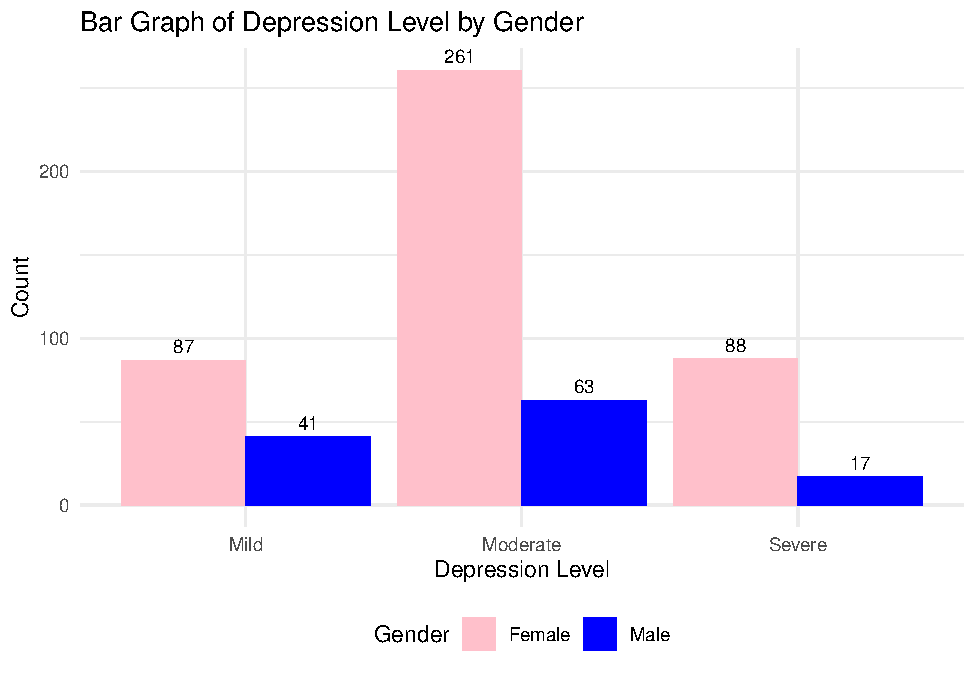
\includegraphics{final_files/figure-latex/gender-depression-bar-1.pdf}
\caption{\label{fig:gender-depression-bar}Bar Graph of Depression Level by Gender}
\end{figure}

\begin{figure}
\centering
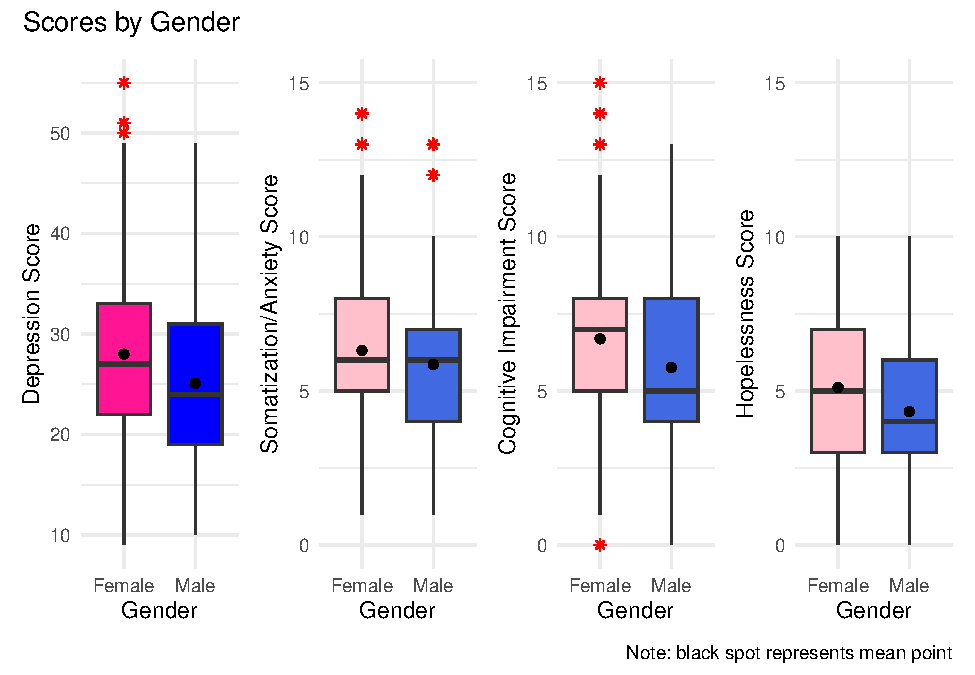
\includegraphics{final_files/figure-latex/boxplot-score-gender-1.pdf}
\caption{\label{fig:boxplot-score-gender}The Combined Descriptive Boxplot of Scores by Gender}
\end{figure}

\begin{table}[tbp]

\begin{center}
\begin{threeparttable}

\caption{\label{tab:table-mean-gender}Mean Scores by Gender}

\begin{tabular}{lll}
\toprule
Mean & \multicolumn{1}{c}{Male} & \multicolumn{1}{c}{Female}\\
\midrule
Depression Score & 25.10 & 28.00\\
Anxiety/Somatic Score & 5.86 & 6.31\\
Cognitive Impairment Score & 5.76 & 6.69\\
Hopelessness Score & 4.33 & 5.11\\
\bottomrule
\end{tabular}

\end{threeparttable}
\end{center}

\end{table}

Meanwhile, the Table \ref{tab:table-mean-gender} presents a more direct gender differences in mean where the mean of depression score for males is 25.10 lower than female's, which is 28. Meanwhile, female adolescents have higher mean in somatization/anxiety scores (6.31), cognitive impairment score (6.69), as well as hopelessness score (5.11) compared to male adolescents who have a mean somatization/anxiety score of 5.86, a cognitive impairment score of 5.76, and a hopelessness score of 4.33.

\hypertarget{statistic-analysis}{%
\subsection{Statistic Analysis}\label{statistic-analysis}}

We used R (Version 4.3.2; R Core Team, 2023) and the R-packages \emph{broom} (Version 1.0.5; Robinson, Hayes, \& Couch, 2023), \emph{car} (Version 3.1.2; Fox \& Weisberg, 2019; Fox, Weisberg, \& Price, 2022), \emph{carData} (Version 3.0.5; Fox et al., 2022), \emph{citr} (Version 0.3.2; Aust, 2019), \emph{dplyr} (Version 1.1.4; Wickham, François, Henry, Müller, \& Vaughan, 2023), \emph{forcats} (Version 1.0.0; Wickham, 2023a), \emph{ggplot2} (Version 3.4.4; Wickham, 2016), \emph{lubridate} (Version 1.9.3; Grolemund \& Wickham, 2011), \emph{papaja} (Version 0.1.2; Aust \& Barth, 2023), \emph{patchwork} (Version 1.2.0; Pedersen, 2024), \emph{purrr} (Version 1.0.2; Wickham \& Henry, 2023), \emph{readr} (Version 2.1.4; Wickham, Hester, \& Bryan, 2023), \emph{readxl} (Version 1.4.3; Wickham \& Bryan, 2023), \emph{Require} (Version 0.3.1; McIntire, 2023), \emph{rmarkdown} (Version 2.25; Xie, Allaire, \& Grolemund, 2018; Xie, Dervieux, \& Riederer, 2020), \emph{shiny} (Version 1.8.0; Chang et al., 2023), \emph{stringr} (Version 1.5.1; Wickham, 2023b), \emph{tibble} (Version 3.2.1; Müller \& Wickham, 2023), \emph{tidyr} (Version 1.3.0; Wickham, Vaughan, \& Girlich, 2023), \emph{tidyverse} (Version 2.0.0; Wickham et al., 2019), \emph{tinylabels} (Version 0.2.4; Barth, 2023), and \emph{writexl} (Version 1.4.2; Ooms, 2023) for references.

\begin{table}[tbp]

\begin{center}
\begin{threeparttable}

\caption{\label{tab:regression-depression-gender}Regression Analysis of Depression Scores by Gender}

\begin{tabular}{lllll}
\toprule
term & \multicolumn{1}{c}{estimate} & \multicolumn{1}{c}{std.error} & \multicolumn{1}{c}{statistic} & \multicolumn{1}{c}{p.value}\\
\midrule
(Intercept) & 28.00 & 0.42 & 67.07 & < .001\\
GenderMale & -2.90 & 0.90 & -3.24 & < .01\\
\bottomrule
\addlinespace
\end{tabular}

\begin{tablenotes}[para]
\normalsize{\textit{Note.} This table presents the output of a linear regression model with Depression Score as the outcome and Gender as the predictor.P values are reported as '< .01' for values between .001 and .01, and as '< .001' for values less than .001.}
\end{tablenotes}

\end{threeparttable}
\end{center}

\end{table}

The regression analysis was performed to examine the impact of gender on depression scores. As Table \ref{tab:regression-depression-gender} indicates, there was a statistically significant difference in depression scores by gender, with males showing lower depression scores compared to females (\(\beta\) = -2.90, t = -3.24, p \textless{} .01).

\begin{table}[tbp]

\begin{center}
\begin{threeparttable}

\caption{\label{tab:ttest-scores-gender}T-test Results for Scores by Gender}

\begin{tabular}{llll}
\toprule
 & \multicolumn{1}{c}{t.value} & \multicolumn{1}{c}{df} & \multicolumn{1}{c}{p.value}\\
\midrule
Depression Score & 3.29 & 196.50 & < .01\\
Somatization/Anxiety Score & 1.88 & 191.46 & 0.06\\
Cognitive Impairment Score & 3.06 & 192.57 & < .01\\
Hopelessness Score & 3.40 & 197.11 & < .001\\
\bottomrule
\addlinespace
\end{tabular}

\begin{tablenotes}[para]
\normalsize{\textit{Note.} This table includes t values, degrees of freedom (df), and p values for the comparison of scores by gender. P values are reported as '< .01' for values between .001 and .01, and as '< .001' for values less than .001.}
\end{tablenotes}

\end{threeparttable}
\end{center}

\end{table}

The t-tests were conducted to assess the gender differences in depression scores and three symptoms' scores. The results indicated that females had higher mean scores compared to males in all categories, aligning with Table \ref{tab:table-mean-gender}. Specificly, females reported significantly higher levels of depression, showing by the tatal HAM-D depression score, than males, t( 196.50) = 3.29, p \textless{} .01.
Meanwhile, Cognitive impairment scores were significantly higher for females(t(192.57) = 3.06, p \textless{} .01). Also, a significant difference in hopelessness scores was also found, where (t(197.11) = 3.40, p \textless{} .001), with females experiencing higher levels of hopelessness.''
However, the trend for higher somatization/anxiety in females was noted, but the result of t-test was not statistically significant, where (t(191.46) = 1.88, p = 0.06), greater than .05 (see Table \ref{tab:ttest-scores-gender}).

\hypertarget{discussion}{%
\section{Discussion}\label{discussion}}

The statstic findings mostly align with our expectations, showing that female adolescents with depression exhibit a higher severity of depression and more pronounced symptoms of cognitive impairment and hopelessness compared to their male peers. These results partly reveal the higher vulnerability of female adolescents, suggesting the need for more targeted clinical treatments based on gender differences. Future studies should explore topics such as whether certain cultural values or gender stereotypes in China contribute to this vulnerability in female adolescents, as well as potential resilience factors.

At the same time, the independent test on gender differences in somatization/anxiety reported an insignificant. Our study has a limitation in that the number of female patients significantly exceeds that of male patients, which might have contributed to the non-significant findings in the gender differences for the somatization/anxiety depressive factor. Additionally, the definition of the somatization/anxiety factor in our study, based on the HAM-D-24, might differ from other studies that assess gender differences in somatic symptoms. For example, the study by Silverstein (1995) includes disordered eating and headache in its definition of anxiety and somatic symptomatology, whereas our study incorporates a broader range of items such as hypochondria and insights, along with headache as a general somatic symptom. Therefore, further research on gender differences in somatization/anxiety depressive symptoms is warranted to explain the inconsistencies observed different related studies.

As a sub-study of depression in Chinese adolescents, this research provides background information and analytical reference for the larger study, revealing gender differences in adolescent depression in China. This contributes to a more comprehensive understanding of this mental illness in this age group within a non-Western context. Gender differences in other depressive symptoms, as well as the occurrence and severity of depression and depressive symptoms across different adolescent age groups (10-13, 14-17, and 18-19 years), will be explored in subsequent sub-studies. Originating from the study of Depression in Chinese Adolescents, this research aims to contribute to the development of a culture-specific psychological treatment system for patients that fits our cultural context.

\hypertarget{limitations}{%
\subsection{Limitations}\label{limitations}}

Our study's limitations include a notable number imbalance with more female than male participants, potentially biasing the analysis of gender differences. This overrepresentation could distort the observed effects of depression. Additionally, our reliance on binary sex categorization did not consider participants' self-identified gender, potentially overlooking the nuances between biological sex and gender identity. Future research should aim for more gender-balanced samples and consider a broader spectrum of gender identities to enhance our understanding of depression in adolescents.

\newpage

\hypertarget{reference}{%
\section{Reference}\label{reference}}

\hypertarget{ref}{}

\hypertarget{refs}{}
\begin{CSLReferences}{1}{0}
\leavevmode\vadjust pre{\hypertarget{ref-alloy1987depression}{}}%
Alloy, L. B., \& Ahrens, A. H. (1987). Depression and pessimism for the future: Biased use of statistically relevant information in predictions for self versus others. \emph{Journal of Personality and Social Psychology}, \emph{52}(2), 366.

\leavevmode\vadjust pre{\hypertarget{ref-R-citr}{}}%
Aust, F. (2019). \emph{Citr: 'RStudio' add-in to insert markdown citations}. Retrieved from \url{https://github.com/crsh/citr}

\leavevmode\vadjust pre{\hypertarget{ref-R-papaja}{}}%
Aust, F., \& Barth, M. (2023). \emph{{papaja}: {Prepare} reproducible {APA} journal articles with {R Markdown}}. Retrieved from \url{https://github.com/crsh/papaja}

\leavevmode\vadjust pre{\hypertarget{ref-R-tinylabels}{}}%
Barth, M. (2023). \emph{{tinylabels}: Lightweight variable labels}. Retrieved from \url{https://cran.r-project.org/package=tinylabels}

\leavevmode\vadjust pre{\hypertarget{ref-beck1993hopelessness}{}}%
Beck, A. T., Steer, R. A., Beck, J. S., \& Newman, C. F. (1993). Hopelessness, depression, suicidal ideation, and clinical diagnosis of depression. \emph{Suicide and Life-Threatening Behavior}, \emph{23}(2), 139--145.

\leavevmode\vadjust pre{\hypertarget{ref-blakemore_is_2014}{}}%
Blakemore, S.-J., \& Mills, K. L. (2014). Is {Adolescence} a {Sensitive} {Period} for {Sociocultural} {Processing}? \emph{Annual Review of Psychology}, \emph{65}(1), 187--207. \url{https://doi.org/10.1146/annurev-psych-010213-115202}

\leavevmode\vadjust pre{\hypertarget{ref-R-shiny}{}}%
Chang, W., Cheng, J., Allaire, J., Sievert, C., Schloerke, B., Xie, Y., \ldots{} Borges, B. (2023). \emph{Shiny: Web application framework for r}. Retrieved from \url{https://CRAN.R-project.org/package=shiny}

\leavevmode\vadjust pre{\hypertarget{ref-clayborne_systematic_2019}{}}%
Clayborne, Z. M., Varin, M., \& Colman, I. (2019). Systematic {Review} and {Meta}-{Analysis}: {Adolescent} {Depression} and {Long}-{Term} {Psychosocial} {Outcomes}. \emph{Journal of the American Academy of Child \& Adolescent Psychiatry}, \emph{58}(1), 72--79. \url{https://doi.org/10.1016/j.jaac.2018.07.896}

\leavevmode\vadjust pre{\hypertarget{ref-R-car}{}}%
Fox, J., \& Weisberg, S. (2019). \emph{An {R} companion to applied regression} (Third). Thousand Oaks {CA}: Sage. Retrieved from \url{https://socialsciences.mcmaster.ca/jfox/Books/Companion/}

\leavevmode\vadjust pre{\hypertarget{ref-R-carData}{}}%
Fox, J., Weisberg, S., \& Price, B. (2022). \emph{carData: Companion to applied regression data sets}. Retrieved from \url{https://CRAN.R-project.org/package=carData}

\leavevmode\vadjust pre{\hypertarget{ref-R-lubridate}{}}%
Grolemund, G., \& Wickham, H. (2011). Dates and times made easy with {lubridate}. \emph{Journal of Statistical Software}, \emph{40}(3), 1--25. Retrieved from \url{https://www.jstatsoft.org/v40/i03/}

\leavevmode\vadjust pre{\hypertarget{ref-hamilton_rating_1960}{}}%
Hamilton, M. (1960). A {Rating} {Scale} for {Depression}. \emph{Journal of Neurology, Neurosurgery, and Psychiatry}, \emph{23}(1), 56--62. Retrieved from \url{https://www.ncbi.nlm.nih.gov/pmc/articles/PMC495331/}

\leavevmode\vadjust pre{\hypertarget{ref-heidari_sex_2016}{}}%
Heidari, S., Babor, T. F., De Castro, P., Tort, S., \& Curno, M. (2016). Sex and {Gender} {Equity} in {Research}: Rationale for the {SAGER} guidelines and recommended use. \emph{Research Integrity and Peer Review}, \emph{1}(1), 2. \url{https://doi.org/10.1186/s41073-016-0007-6}

\leavevmode\vadjust pre{\hypertarget{ref-hesketh_anxiety_2005}{}}%
Hesketh, T., \& Ding, Q. J. (2005). Anxiety and {Depression} in {Adolescents} in {Urban} and {Rural} {China}. \emph{Psychological Reports}, \emph{96}(2), 435--444. \url{https://doi.org/10.2466/pr0.96.2.435-444}

\leavevmode\vadjust pre{\hypertarget{ref-jung_association_2019}{}}%
Jung, S. J., Cho, S. M. J., \& Kim, H. C. (2019). Association of oral contraceptive use with suicidal behavior among representative {Korean} population: {Results} from {Korea} {National} {Health} and {Nutrition} {Examination} {Survey} (2007--2016). \emph{Journal of Affective Disorders}, \emph{243}, 8--15. \url{https://doi.org/10.1016/j.jad.2018.09.004}

\leavevmode\vadjust pre{\hypertarget{ref-lam2014cognitive}{}}%
Lam, R. W., Kennedy, S. H., McIntyre, R. S., \& Khullar, A. (2014). Cognitive dysfunction in major depressive disorder: Effects on psychosocial functioning and implications for treatment. \emph{The Canadian Journal of Psychiatry}, \emph{59}(12), 649--654.

\leavevmode\vadjust pre{\hypertarget{ref-lewis_gender_2015}{}}%
Lewis, A. J., Kremer, P., Douglas, K., Toumborou, J. W., Hameed, M. A., Patton, G. C., \& Williams, J. (2015). Gender differences in adolescent depression: {Differential} female susceptibility to stressors affecting family functioning. \emph{Australian Journal of Psychology}, \emph{67}(3), 131--139. \url{https://doi.org/10.1111/ajpy.12086}

\leavevmode\vadjust pre{\hypertarget{ref-lipowski1990somatization}{}}%
Lipowski, Z. J. (1990). Somatization and depression. \emph{Psychosomatics}, \emph{31}(1), 13--21.

\leavevmode\vadjust pre{\hypertarget{ref-lv2023sex}{}}%
Lv, Q., Li, X., Zhang, Y., Lu, D., Lu, J., Xie, Q., \ldots{} Yi, Z. (2023). Sex differences in subjective cognitive impairment and clinical correlates in chinese patients with subthreshold depression. \emph{Biology of Sex Differences}, \emph{14}(1), 6.

\leavevmode\vadjust pre{\hypertarget{ref-R-Require}{}}%
McIntire, E. J. B. (2023). \emph{Require: Installing and loading r packages for reproducible workflows}. Retrieved from \url{https://CRAN.R-project.org/package=Require}

\leavevmode\vadjust pre{\hypertarget{ref-R-tibble}{}}%
Müller, K., \& Wickham, H. (2023). \emph{Tibble: Simple data frames}. Retrieved from \url{https://CRAN.R-project.org/package=tibble}

\leavevmode\vadjust pre{\hypertarget{ref-NIMH_Depression_2023}{}}%
NIMH. (2023). \emph{Depressive disorder (depression)}. National Institute of Mental Health. Retrieved from \url{http://www.who.int/mediacentre/factsheets/fs369/en/}

\leavevmode\vadjust pre{\hypertarget{ref-nolen1990sex}{}}%
Nolen-Hoeksema, S. (1990). \emph{Sex differences in depression}. Stanford University Press.

\leavevmode\vadjust pre{\hypertarget{ref-nolen2013handbook}{}}%
Nolen-Hoeksema, S., \& Hilt, L. M. (2013). \emph{Handbook of depression in adolescents}. Routledge.

\leavevmode\vadjust pre{\hypertarget{ref-R-writexl}{}}%
Ooms, J. (2023). \emph{Writexl: Export data frames to excel 'xlsx' format}. Retrieved from \url{https://CRAN.R-project.org/package=writexl}

\leavevmode\vadjust pre{\hypertarget{ref-R-patchwork}{}}%
Pedersen, T. L. (2024). \emph{Patchwork: The composer of plots}. Retrieved from \url{https://CRAN.R-project.org/package=patchwork}

\leavevmode\vadjust pre{\hypertarget{ref-quach_effects_2015}{}}%
Quach, A. S., Epstein, N. B., Riley, P. J., Falconier, M. K., \& Fang, X. (2015). Effects of {Parental} {Warmth} and {Academic} {Pressure} on {Anxiety} and {Depression} {Symptoms} in {Chinese} {Adolescents}. \emph{Journal of Child and Family Studies}, \emph{24}(1), 106--116. \url{https://doi.org/10.1007/s10826-013-9818-y}

\leavevmode\vadjust pre{\hypertarget{ref-R-base}{}}%
R Core Team. (2023). \emph{R: A language and environment for statistical computing}. Vienna, Austria: R Foundation for Statistical Computing. Retrieved from \url{https://www.R-project.org/}

\leavevmode\vadjust pre{\hypertarget{ref-R-broom}{}}%
Robinson, D., Hayes, A., \& Couch, S. (2023). \emph{Broom: Convert statistical objects into tidy tibbles}. Retrieved from \url{https://CRAN.R-project.org/package=broom}

\leavevmode\vadjust pre{\hypertarget{ref-silverstein1995gender}{}}%
Silverstein, B., Caceres, J., Perdue, L., \& Cimarolli, V. (1995). Gender differences in depressive symptomatology: The role played by {``anxious somatic depression''} associated with gender-related achievement concerns. \emph{Sex Roles}, \emph{33}, 621--636.

\leavevmode\vadjust pre{\hypertarget{ref-sun_more_2023}{}}%
Sun, Y., Zhong, Y., Sun, W., Chu, L., Long, J., \& Fan, X. W. (2023). More prevalent and more severe: Gender differences of depressive symptoms in {Chinese} adolescents. \emph{Frontiers in Public Health}, \emph{11}. Retrieved from \url{https://www.frontiersin.org/journals/public-health/articles/10.3389/fpubh.2023.1167234}

\leavevmode\vadjust pre{\hypertarget{ref-takacs2023large}{}}%
Takács, J., Katona, Z. B., \& Ihász, F. (2023). A large sample cross-sectional study on mental health challenges among adolescents and young adults during the COVID-19 pandemic at-risk group for loneliness and hopelessness during the COVID-19 pandemic. \emph{Journal of Affective Disorders}, \emph{325}, 770--777.

\leavevmode\vadjust pre{\hypertarget{ref-WHO_Depression_2017}{}}%
WHO. (2017). \emph{Depressive disorder (depression)}. World Health Organization. Retrieved from \url{http://www.who.int/mediacentre/factsheets/fs369/en/}

\leavevmode\vadjust pre{\hypertarget{ref-R-ggplot2}{}}%
Wickham, H. (2016). \emph{ggplot2: Elegant graphics for data analysis}. Springer-Verlag New York. Retrieved from \url{https://ggplot2.tidyverse.org}

\leavevmode\vadjust pre{\hypertarget{ref-R-forcats}{}}%
Wickham, H. (2023a). \emph{Forcats: Tools for working with categorical variables (factors)}. Retrieved from \url{https://CRAN.R-project.org/package=forcats}

\leavevmode\vadjust pre{\hypertarget{ref-R-stringr}{}}%
Wickham, H. (2023b). \emph{Stringr: Simple, consistent wrappers for common string operations}. Retrieved from \url{https://CRAN.R-project.org/package=stringr}

\leavevmode\vadjust pre{\hypertarget{ref-R-tidyverse}{}}%
Wickham, H., Averick, M., Bryan, J., Chang, W., McGowan, L. D., François, R., \ldots{} Yutani, H. (2019). Welcome to the {tidyverse}. \emph{Journal of Open Source Software}, \emph{4}(43), 1686. \url{https://doi.org/10.21105/joss.01686}

\leavevmode\vadjust pre{\hypertarget{ref-R-readxl}{}}%
Wickham, H., \& Bryan, J. (2023). \emph{Readxl: Read excel files}. Retrieved from \url{https://CRAN.R-project.org/package=readxl}

\leavevmode\vadjust pre{\hypertarget{ref-R-dplyr}{}}%
Wickham, H., François, R., Henry, L., Müller, K., \& Vaughan, D. (2023). \emph{Dplyr: A grammar of data manipulation}. Retrieved from \url{https://CRAN.R-project.org/package=dplyr}

\leavevmode\vadjust pre{\hypertarget{ref-R-purrr}{}}%
Wickham, H., \& Henry, L. (2023). \emph{Purrr: Functional programming tools}. Retrieved from \url{https://CRAN.R-project.org/package=purrr}

\leavevmode\vadjust pre{\hypertarget{ref-R-readr}{}}%
Wickham, H., Hester, J., \& Bryan, J. (2023). \emph{Readr: Read rectangular text data}. Retrieved from \url{https://CRAN.R-project.org/package=readr}

\leavevmode\vadjust pre{\hypertarget{ref-R-tidyr}{}}%
Wickham, H., Vaughan, D., \& Girlich, M. (2023). \emph{Tidyr: Tidy messy data}. Retrieved from \url{https://CRAN.R-project.org/package=tidyr}

\leavevmode\vadjust pre{\hypertarget{ref-R-rmarkdown_a}{}}%
Xie, Y., Allaire, J. J., \& Grolemund, G. (2018). \emph{R markdown: The definitive guide}. Boca Raton, Florida: Chapman; Hall/CRC. Retrieved from \url{https://bookdown.org/yihui/rmarkdown}

\leavevmode\vadjust pre{\hypertarget{ref-R-rmarkdown_b}{}}%
Xie, Y., Dervieux, C., \& Riederer, E. (2020). \emph{R markdown cookbook}. Boca Raton, Florida: Chapman; Hall/CRC. Retrieved from \url{https://bookdown.org/yihui/rmarkdown-cookbook}

\end{CSLReferences}


\end{document}
